\section{Valeur, direction et sens (3 points)}

Quatre vitesses d'objets à un moment précis sont représentées ci-dessous.

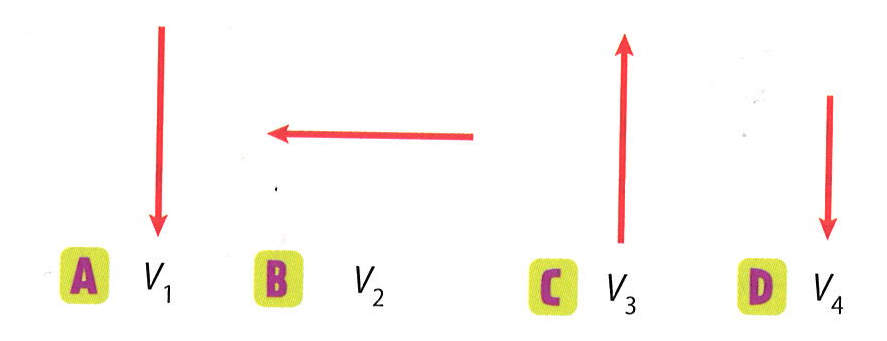
\includegraphics[scale=0.5]{exemples}

\begin{questions}
	\question \'A l'instant représenté, quels objets ont :
	\begin{parts}
		\part[1] la même direction ?
		\fillwithdottedlines{1.5cm}
		
		\part[1] le même sens de déplacement ?
		\fillwithdottedlines{1.5cm}
		
		\part[1] la même valeur ?
		\fillwithdottedlines{1.5cm}
	\end{parts}

\end{questions}